\let\negmedspace\undefined
\let\negthickspace\undefined
\documentclass[journal]{IEEEtran}
\usepackage[a5paper, margin=10mm, onecolumn]{geometry}
\usepackage{lmodern} % Ensure lmodern is loaded for pdflatex
\usepackage{tfrupee} % Include tfrupee package

\setlength{\headheight}{1cm} % Set the height of the header box
\setlength{\headsep}{0mm}     % Set the distance between the header box and the top of the text

\usepackage{gvv-book}
\usepackage{gvv}
\usepackage{cite}
\usepackage{amsmath,amssymb,amsfonts,amsthm}
\usepackage{algorithmic}
\usepackage{graphicx}
\usepackage{textcomp}
\usepackage{xcolor}
\usepackage{txfonts}
\usepackage{listings}
\usepackage{enumitem}
\usepackage{mathtools}
\usepackage{gensymb}
\usepackage{comment}
\usepackage[breaklinks=true]{hyperref}
\usepackage{tkz-euclide} 
\usepackage{listings}                                      
\def\inputGnumericTable{}                                 
\usepackage[latin1]{inputenc}                                
\usepackage{color}                                            
\usepackage{array}                                            
\usepackage{longtable}
\usepackage{multicol}
\usepackage{calc}                                             
\usepackage{multirow}                                         
\usepackage{hhline}                                           
\usepackage{ifthen}                                           
\usepackage{lscape}

\begin{document}

\bibliographystyle{IEEEtran}
\vspace{3cm}

\title{Lab-1 Report}
\author{EE24BTECH11024, EE24BTECH11002}
{\let\newpage\relax\maketitle}

\renewcommand{\thefigure}{\theenumi}
\renewcommand{\thetable}{\theenumi}
\setlength{\intextsep}{10pt} % Space between text and floats

\numberwithin{equation}{enumi}
\numberwithin{figure}{enumi}
\renewcommand{\thetable}{\theenumi}

\section*{Connecting the Oscilloscope}
To connect the osciiloscope to function generator properly do the following -
\begin{itemize}
    \item Connect one probe (probe A) to the wire connected to the output terminal of Channel 1 in function generator, and connect the ground of the probe A to the ground of channel 1, do the same to the second probe (probe B).
    \item Set both the probes to 10x condition and in the oscilloscope. 
    \item Use the triggering feature to lock the waveform for analysis.
\end{itemize}

\section*{Using a Function Generator}
A function generator produces various types of periodic signals, such as sine, square, and triangular waveforms. It is often used to test circuits by providing known input signals. Key steps in its operation include:
\begin{enumerate}
    \item \textbf{Setting the Waveform}: Select the desired waveform type (e.g., sine wave) using the function generator's interface.
    \item \textbf{Adjusting Frequency and Amplitude}: Use the control knobs to set the required frequency and amplitude for the waveform.
    \item \textbf{Connecting to the Circuit}: Attach the output terminals to the circuit or oscilloscope input for signal injection.
\end{enumerate}
The function generator complements the oscilloscope by providing a controllable input signal for testing and analysis.

\section*{Results}
\begin{figure}[h!]
   \centering
   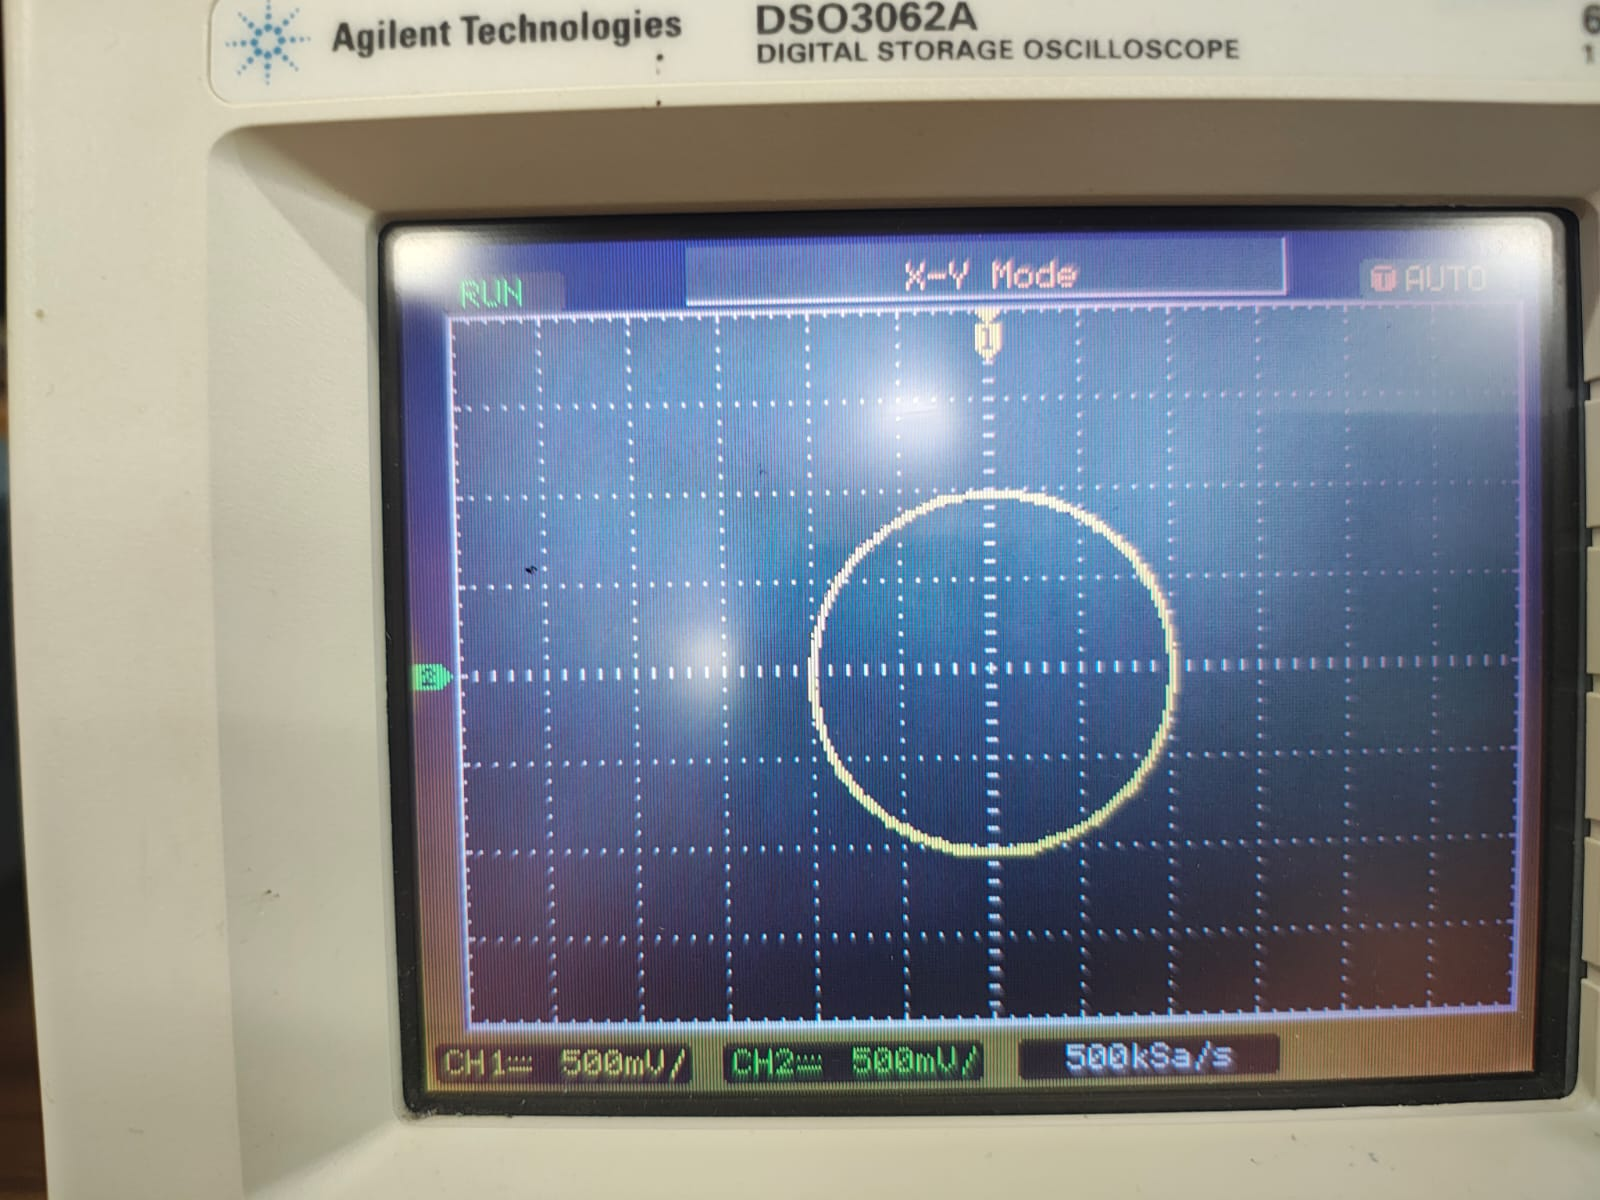
\includegraphics[width=\columnwidth]{figs/fig1.png}
   \caption{Comparison between the Theoretical solution and Computational solution}
   \label{stemplot}
\end{figure}

Figure \ref{stemplot} illustrates the comparison between the theoretical solution and the computational solution. The oscilloscope and function generator were instrumental in verifying the experimental results.

\section*{Conclusion}
This lab session demonstrated the effective use of an oscilloscope and function generator in analyzing and verifying circuit behaviors. Mastery of these tools is essential for accurate experimental validation in electrical engineering.

\end{document}

